\documentclass{article}
  %----------------------------------------------------------------------------------------
%	Author:	WangYifu
%	Create Date:	2017-02-14
%	Last Modify:	2018-09-01
%----------------------------------------------------------------------------------------
\usepackage[T1]{fontenc}
\usepackage{fourier}
\usepackage[english]{babel}
\usepackage{amsmath,amsfonts,amsthm}
\usepackage{geometry}
\usepackage{fancyhdr}
\usepackage{listings}
\usepackage{color}
\usepackage[yyyymmdd]{datetime}
\usepackage{graphicx}
\usepackage{float}
\usepackage{titling}
\usepackage{titlesec}
%-------------------------------%
%          Page Style           %
%-------------------------------%
\pagestyle{fancyplain}
\fancyhead{}
\fancyfoot[L]{}
\fancyfoot[C]{}
\fancyfoot[R]{\thepage}
\renewcommand{\headrulewidth}{0pt}
\renewcommand{\footrulewidth}{0pt}
\setlength{\headheight}{13.6pt}
\textwidth=6.5in
\textheight=9.0in
\headsep = 0.1in
\renewcommand{\baselinestretch}{1.2}
\geometry{a4paper,left=2cm,right=2cm,top=2cm,bottom=2cm}

%-------------------------------%
%           Font Size           %
%-------------------------------%
\newcommand{\erhao}{\fontsize{22.1pt}{\baselineskip}\selectfont}
\newcommand{\sanhao}{\fontsize{16.1pt}{\baselineskip}\selectfont}
\newcommand{\sihao}{\fontsize{14.1pt}{\baselineskip}\selectfont}
\newcommand{\xiaosi}{\fontsize{12.1pt}{\baselineskip}\selectfont}
\newcommand{\wuhao}{\fontsize{10.5pt}{\baselineskip}\selectfont}
\newcommand{\setFontSize}[1]{\fontsize{#1}{\baselineskip}\selectfont}
\titleformat{\section}{\sanhao\bfseries}{$\bullet$}{5pt}{}

%-------------------------------%
%             Title             %
%-------------------------------%
\newcommand{\horrule}[1]{\rule{\linewidth}{#1}}
\renewcommand{\dateseparator}{ - }
\def\Assignment{Assignment Title}
\title{
\vspace{-2cm}
\normalfont \normalsize
\textsc{Washington University in St. Louis} \\ [0pt]
\horrule{1pt} \\[0.4cm]
\huge {\bf\Assignment}
}
\author{467261 - Yifu Wang}
\date{\normalsize\today\\\horrule{1pt} \\[0.5cm]}

%-------------------------------%
%           TableList           %
%-------------------------------%
\newcommand{\deflabel}[1]{#1\hfill}
\newenvironment{tlist}[1]{
	\begin{list}{}{
			\settowidth{\labelwidth}{\bf#1}
			\setlength{\leftmargin}{\labelwidth}
			\addtolength{\leftmargin}{\labelsep}
			\renewcommand{\makelabel}{\bf\deflabel}}}{
	\end{list}
}

%-------------------------------%
%             Code              %
%-------------------------------%
\definecolor{gray}{RGB}{191,191,191}
\definecolor{dkgreen}{RGB}{96,139,78}
\definecolor{mauve}{RGB}{206,145,120}

\lstset{ %
	language=C++,                % the language of the code
	% basicstyle=\textheight,           % the size of the fonts that are used for the code
	numbers=left,                   % where to put the line-numbers
	numberstyle=\color{black},  % the style that is used for the line-numbers
	stepnumber=0,                   % the step between two line-numbers. If it's 1, each line 
	% will be numbered
	numbersep=5pt,                  % how far the line-numbers are from the code
	backgroundcolor=\color{gray},      % choose the background color. You must add \usepackage{color}
	showspaces=false,               % show spaces adding particular underscores
	showstringspaces=false,         % underline spaces within strings
	showtabs=false,                 % show tabs within strings adding particular underscores
	frame=false,                   % adds a frame around the code
	rulecolor=\color{gray},        % if not set, the frame-color may be changed on line-breaks within not-black text (e.g. commens (green here))
	tabsize=2,                      % sets default tabsize to 2 spaces
	captionpos=b,                   % sets the caption-position to bottom
	breaklines=true,                % sets automatic line breaking
	breakatwhitespace=false,        % sets if automatic breaks should only happen at whitespace
	keywordstyle=\color{blue},          % keyword style
	commentstyle=\color{dkgreen},       % comment style
	stringstyle=\color{mauve},         % string literal style
}

  \def\Assignment{CSE 417T - HW2}
  \def\mH{m_\mathcal{H}}
\begin{document}
\maketitle
\begin{tlist}{5}
	\item[1.12]
	\begin{tlist}{4}
		\item[(a)]
		Denote $h_{mean}$ as $\bar{y}$. To prove $\bar{y}$ makes $E_{in}(h)$ minimal. Basically we only need to show $E_{in}(h) \geq E_{in}(\bar{y})$. Which is obviously since $E'_{in}(h)=2\sum^N_{n=1}(h-y_n)=2N(h-\bar{y})$, when $h<\bar{y}$ $E'<0$, when $h>\bar{y}$ $E'>0$, thus $E$ reach its minimal value at $\bar{y}$. \qed
		\item[(b)]
		We try to calculate the derivative of $E$ as we did in \textbf{(a)} but since $E$ is sum of absolutes, we can redefine $E$ to get rid of absolute.
		$$E_{in}(h)=\begin{cases}
				\sum_{n=1}^N (y_n-h)
				 & h \leq y_1                                \\
				\sum_{n=1}^i (h-y_n) + \sum_{n=i+1}^N (y_n-h)
				 & y_{i} \leq h \leq y_{i+1}\ ,\ i\in[1,n-1] \\
				\sum_{n=1}^N (h-y_n)
				 & h \geq y_N
			\end{cases}$$
		Thus we have
		$$E'_{in}(h)=\begin{cases}
				-N   & h \leq y_1                                \\
				2i-N & y_{i} \leq h \leq y_{i+1}\ ,\ i\in[1,n-1] \\
				N    & h \geq y_N
			\end{cases}$$
		$E'$ is a monotonically decreasing function, and by the definition of $h_{med}$, $E'$ will reach its zero point at $h_{med}$. Namely, $E$ will reach its minimal value at $h_{med}$. \qed\\
		And notice that $h_{med}$ will be a single value only if $N$ is odd.
		\item[(c)]
		$h_{mean}$ will tend to $\infty$ in all condition.\\
		$h_{med}$ will tend to $\infty$ if $N \leq 2$, will remain same otherwise.
	\end{tlist}
	\item[2.3]
	\begin{tlist}{4}
		\item[(a)]
		Giving $N$ points, $\mathbb{R}$ will be divide into $N+1$ interval (assume no coincided since we just need the max value). The result of positive or negative ray is totaly depends on which interval contains $a$. Considering $a\in (-\infty,X_1)\cup (X_N,\infty)$, only two results will be produced all $+1$ and all $-1$. Thus $m_{\mathcal{H}}(N)=2(N-1)+2=2N$, $d_{VC}=2$.\qed
		\item[(b)]
		Firstly consider positive interval only, if at one $X_i$ locate inside the interval $[a,b]$ then $a$ and $b$ must locate in different interval divided by $X$, which produce $(N+1)N/2$ results. Plus the all $-1$ condition that should be the max number of dichotomies of positive intervals. Take negative intervals into consider, the only thing we need to pay attention is the following situation. Denote a positive interval as $[a_1,b_1]$ and a negative interval as $[a_2,b_2]$. If $a_1 < X_1$ $b_2 > X_N$ and $b_1,a_1\in [X_i,X_{i+1}]$. These two interval will produce same results. Thus $m_{\mathcal{H}}(N)=(2+N)(N-1)-2(N-1)+2=N^2-N+2$, $d_{VC}=3$.\qed
		\item[(c)]
		This is equivalent to positive interval with $\mathcal{X}=[0,\infty)$ and $a,b\geq 0$, which won't affect the result. Thus $\mH(N)=N(N+1)/2+1$, $d_{VC}=2$.\qed
	\end{tlist}
	\item[2.8]
	A valid growth function $\mH(N)$ should firstly satisfy $\forall N\in\mathbb{N^+}, \mH(N)\leq 2^N$, then $\forall k \text{ satisfy } \mH(k)<2^k, \mH(N)\leq\sum_{i=0}^{k-1}C^i_N\forall N\in\mathbb{N^+}$. Thus once we find the $d_{VC}$ we find the lower bound.\\
	$\mathbf{1+N\ \text{Good}}$: The $d_{VC}$ is 1.\\
	$\mathbf{1+N+\frac{N(N-1)}{2}\ \text{Good}}$: The $d_{VC}$ is 2.\\
	$\mathbf{2^N\ \text{Good}}$: No break point.\\
	$\mathbf{2^{\lfloor\sqrt{N}\rfloor}\ \text{Bad}}$: The $d_{VC}$ is 1, break its bound when $N\to\infty$.\\
	$\mathbf{2^{\lfloor N/2\rfloor}\ \text{Bad}}$: The $d_{VC}$ is 0, break its bound when $N\to\infty$.\\
	$\mathbf{1+N+\frac{N(N-1)(N-2)}{6}\ \text{Bad}}$: The $d_{VC}$ is 1, break its bound when $N\to\infty$.
	\item[2.10]
	This is actually obvious and almost invole no math. And I thought this derive from a more general formula $$\mH(N_1+N_2)\leq \mH(N_1)\mH(N_2)$$ When taking $N_1=N_2=N$ you get the $\mH(2N)\leq \mH(N)^2$.\\
	Since you could always devide a $N_1+N_2$ size sample into two part size of $N_1$ and $N_2$ if the two parts is independent, you will get $\mH(N_1+N_2)= \mH(N_1)\mH(N_2)$ else you will get $\mH(N_1+N_2)<\mH(N_1)\mH(N_2)$.\qed
	\item[2.13]
	\begin{tlist}{4}
		\item[(a)]
		Since $\mH(N)\leq M$, we have $2^{d_{VC}}\leq M$, namely $d_{VC}\leq \text{log}_2M$.\qed
		\item[(b)]
		$0 \leq d_{VC}(\cap_{k=1}^K \mathcal{H}_k) \leq \max\limits_{1<k<K}d_{VC}(\mathcal{H}_k)$\\
		This result is obvious by the definition of intersection of sets. And when there is no intersection the result will reach the lower bound, when all sets are equale the result will reach the upper bound.\qed
		\item[(c)]
		$\max\limits_{1<k<K}d_{VC}(\mathcal{H}_k) \leq d_{VC}(\cap_{k=1}^K \mathcal{H}_k) \leq \sum\limits_{1<k<K}d_{VC}(\mathcal{H}_k)$\\
		This result is obvious by the definition of union of sets. And when all sets are equale the result will reach the upper bound, when all sets are paire-wise unintersected the result will reach upper bound.\qed
	\end{tlist}
	\item[2.22]
	\def\E{\mathbb{E}}
	\def\D{\mathcal{D}}
	$$\begin{aligned}
			\E_\D[E_\text{out}(g^{(\D)})]
			 & =\ \E_{\D,x,y}[(g^{(\D)}(x)-y(x))^2]                                \\
			 & =\ \E_{\D,x}[(g^{(\D)}(x))^2-2g^{(\D)}(x)\E_y[y(x)]+\E_y[(y(x))^2]] \\
			 & =\ \E_{\D,x}[(g^{(\D)}(x))^2
			-2g^{(\D)}(x)\E_\epsilon[f(x)+\epsilon]
			+\E_\epsilon[(f(x))^2+2\epsilon f(x)+\epsilon^2]]                      \\
			 & =\ \E_{\D,x}[(g^{(\D)}(x))^2-2g^{(\D)}(x)f(x)+(f(x))^2+\sigma^2]    \\
			 & =\ \sigma^2+\text{bias}+\text{var}
		\end{aligned}$$
	\qed
	\item[2.24]
	\begin{tlist}{4}
		\item[(a)]
		$$\begin{aligned}
				\bar{g}(x)
				 & =\ \E_\D[g^{(\D)}(x)]                                  \\
				 & =\ \E_{\{(x_1,x_1^2),(x_2,x_2^2)\}}[(x_1+x_2)x-x_1x_2] \\
				 & =\ 0
			\end{aligned}$$
		\item[(b)]
		Pick up many data sets $\D_i$, calculate $g^{(\D)}(x)$. Then calculate $\bar{g}$ then bias and var then $E_\text{out}$.
		\item[(c)]
		I repeated the experiment for 100,000 times, got
		$$\begin{aligned}
				\text{bias}  & =\ 0.2078                                  \\
				\text{var}   & =\ 0.3371                                  \\
				E_\text{out} & =\ 0.5448\ \approx\ \text{bias}+\text{var} \\
				|g(x)|       & \leq 10^{-3}                               \\
			\end{aligned}$$
		Here is all the result I got in one screenshot, code included. And I upload it to image host, \href{https://i.loli.net/2018/09/30/5bb0ddf829ec4.png}{click here} if you feel the image below is low resolution, or you can zoom in.
		\begin{figure}[H]\centering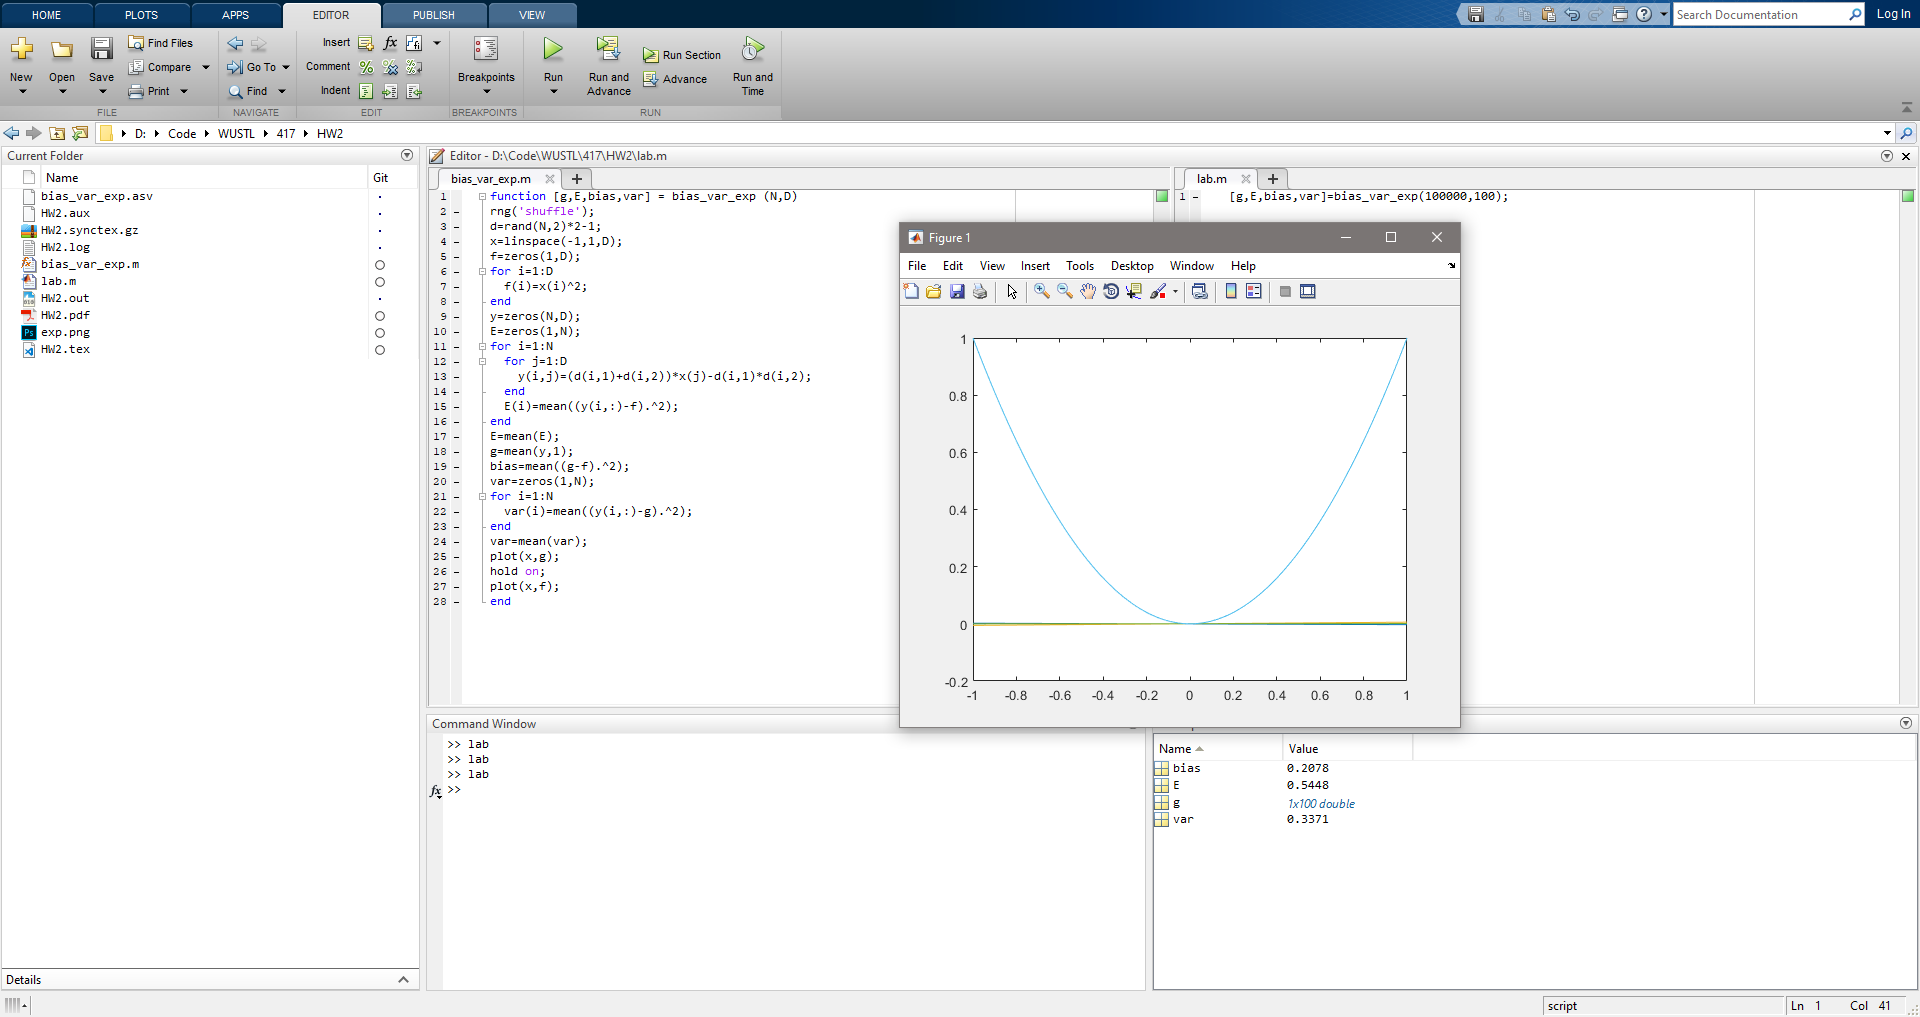
\includegraphics[width=\textwidth]{exp.png}\end{figure}
		\item[(d)]
		Bias
		$$\begin{aligned}
				bias
				 & =\ \E_x[(\bar{g}(x)-f(x))^2]  \\
				 & =\ \E_x[x^4]                  \\
				 & =\ \int_{-1}^1\frac{x^4}{2}dx \\
				 & =\ \frac{1}{5}
			\end{aligned}$$
		Var
		$$\begin{aligned}
				var
				 & =\ \E_{x,\D}[(g^{(\D)}(x)-\bar{g}(x))^2]                                      \\
				 & =\ \int_{-1}^1\int_{-1}^1\int_{-1}^1\frac{1}{8}\frac{3}{2}((y+z)x-yz)^2dzdydx \\
				 & =\ \frac{1}{3}                                                                \\
			\end{aligned}$$
		$\E[E_\text{out}]$
		$$\begin{aligned}
				\E[E_\text{out}]
				 & =\ bias+var     \\
				 & =\ \frac{8}{15}
			\end{aligned}$$
	\end{tlist}
\end{tlist}
\end{document}